% Options for packages loaded elsewhere
\PassOptionsToPackage{unicode}{hyperref}
\PassOptionsToPackage{hyphens}{url}
%
\documentclass[
  ,doc,floatsintext]{apa6}
\usepackage{amsmath,amssymb}
\usepackage{lmodern}
\usepackage{iftex}
\ifPDFTeX
  \usepackage[T1]{fontenc}
  \usepackage[utf8]{inputenc}
  \usepackage{textcomp} % provide euro and other symbols
\else % if luatex or xetex
  \usepackage{unicode-math}
  \defaultfontfeatures{Scale=MatchLowercase}
  \defaultfontfeatures[\rmfamily]{Ligatures=TeX,Scale=1}
\fi
% Use upquote if available, for straight quotes in verbatim environments
\IfFileExists{upquote.sty}{\usepackage{upquote}}{}
\IfFileExists{microtype.sty}{% use microtype if available
  \usepackage[]{microtype}
  \UseMicrotypeSet[protrusion]{basicmath} % disable protrusion for tt fonts
}{}
\makeatletter
\@ifundefined{KOMAClassName}{% if non-KOMA class
  \IfFileExists{parskip.sty}{%
    \usepackage{parskip}
  }{% else
    \setlength{\parindent}{0pt}
    \setlength{\parskip}{6pt plus 2pt minus 1pt}}
}{% if KOMA class
  \KOMAoptions{parskip=half}}
\makeatother
\usepackage{xcolor}
\usepackage{graphicx}
\makeatletter
\def\maxwidth{\ifdim\Gin@nat@width>\linewidth\linewidth\else\Gin@nat@width\fi}
\def\maxheight{\ifdim\Gin@nat@height>\textheight\textheight\else\Gin@nat@height\fi}
\makeatother
% Scale images if necessary, so that they will not overflow the page
% margins by default, and it is still possible to overwrite the defaults
% using explicit options in \includegraphics[width, height, ...]{}
\setkeys{Gin}{width=\maxwidth,height=\maxheight,keepaspectratio}
% Set default figure placement to htbp
\makeatletter
\def\fps@figure{htbp}
\makeatother
\setlength{\emergencystretch}{3em} % prevent overfull lines
\providecommand{\tightlist}{%
  \setlength{\itemsep}{0pt}\setlength{\parskip}{0pt}}
\setcounter{secnumdepth}{-\maxdimen} % remove section numbering
% Make \paragraph and \subparagraph free-standing
\ifx\paragraph\undefined\else
  \let\oldparagraph\paragraph
  \renewcommand{\paragraph}[1]{\oldparagraph{#1}\mbox{}}
\fi
\ifx\subparagraph\undefined\else
  \let\oldsubparagraph\subparagraph
  \renewcommand{\subparagraph}[1]{\oldsubparagraph{#1}\mbox{}}
\fi
\newlength{\cslhangindent}
\setlength{\cslhangindent}{1.5em}
\newlength{\csllabelwidth}
\setlength{\csllabelwidth}{3em}
\newlength{\cslentryspacingunit} % times entry-spacing
\setlength{\cslentryspacingunit}{\parskip}
\newenvironment{CSLReferences}[2] % #1 hanging-ident, #2 entry spacing
 {% don't indent paragraphs
  \setlength{\parindent}{0pt}
  % turn on hanging indent if param 1 is 1
  \ifodd #1
  \let\oldpar\par
  \def\par{\hangindent=\cslhangindent\oldpar}
  \fi
  % set entry spacing
  \setlength{\parskip}{#2\cslentryspacingunit}
 }%
 {}
\usepackage{calc}
\newcommand{\CSLBlock}[1]{#1\hfill\break}
\newcommand{\CSLLeftMargin}[1]{\parbox[t]{\csllabelwidth}{#1}}
\newcommand{\CSLRightInline}[1]{\parbox[t]{\linewidth - \csllabelwidth}{#1}\break}
\newcommand{\CSLIndent}[1]{\hspace{\cslhangindent}#1}
\ifLuaTeX
\usepackage[bidi=basic]{babel}
\else
\usepackage[bidi=default]{babel}
\fi
\babelprovide[main,import]{english}
% get rid of language-specific shorthands (see #6817):
\let\LanguageShortHands\languageshorthands
\def\languageshorthands#1{}
% Manuscript styling
\usepackage{upgreek}
\captionsetup{font=singlespacing,justification=justified}

% Table formatting
\usepackage{longtable}
\usepackage{lscape}
% \usepackage[counterclockwise]{rotating}   % Landscape page setup for large tables
\usepackage{multirow}		% Table styling
\usepackage{tabularx}		% Control Column width
\usepackage[flushleft]{threeparttable}	% Allows for three part tables with a specified notes section
\usepackage{threeparttablex}            % Lets threeparttable work with longtable

% Create new environments so endfloat can handle them
% \newenvironment{ltable}
%   {\begin{landscape}\centering\begin{threeparttable}}
%   {\end{threeparttable}\end{landscape}}
\newenvironment{lltable}{\begin{landscape}\centering\begin{ThreePartTable}}{\end{ThreePartTable}\end{landscape}}

% Enables adjusting longtable caption width to table width
% Solution found at http://golatex.de/longtable-mit-caption-so-breit-wie-die-tabelle-t15767.html
\makeatletter
\newcommand\LastLTentrywidth{1em}
\newlength\longtablewidth
\setlength{\longtablewidth}{1in}
\newcommand{\getlongtablewidth}{\begingroup \ifcsname LT@\roman{LT@tables}\endcsname \global\longtablewidth=0pt \renewcommand{\LT@entry}[2]{\global\advance\longtablewidth by ##2\relax\gdef\LastLTentrywidth{##2}}\@nameuse{LT@\roman{LT@tables}} \fi \endgroup}

% \setlength{\parindent}{0.5in}
% \setlength{\parskip}{0pt plus 0pt minus 0pt}

% Overwrite redefinition of paragraph and subparagraph by the default LaTeX template
% See https://github.com/crsh/papaja/issues/292
\makeatletter
\renewcommand{\paragraph}{\@startsection{paragraph}{4}{\parindent}%
  {0\baselineskip \@plus 0.2ex \@minus 0.2ex}%
  {-1em}%
  {\normalfont\normalsize\bfseries\itshape\typesectitle}}

\renewcommand{\subparagraph}[1]{\@startsection{subparagraph}{5}{1em}%
  {0\baselineskip \@plus 0.2ex \@minus 0.2ex}%
  {-\z@\relax}%
  {\normalfont\normalsize\itshape\hspace{\parindent}{#1}\textit{\addperi}}{\relax}}
\makeatother

% \usepackage{etoolbox}
\makeatletter
\patchcmd{\HyOrg@maketitle}
  {\section{\normalfont\normalsize\abstractname}}
  {\section*{\normalfont\normalsize\abstractname}}
  {}{\typeout{Failed to patch abstract.}}
\patchcmd{\HyOrg@maketitle}
  {\section{\protect\normalfont{\@title}}}
  {\section*{\protect\normalfont{\@title}}}
  {}{\typeout{Failed to patch title.}}
\makeatother

\usepackage{xpatch}
\makeatletter
\xapptocmd\appendix
  {\xapptocmd\section
    {\addcontentsline{toc}{section}{\appendixname\ifoneappendix\else~\theappendix\fi\\: #1}}
    {}{\InnerPatchFailed}%
  }
{}{\PatchFailed}
\keywords{Numerical preference, Social cognition, Avian cognition\newline\indent Word count: }
\usepackage{lineno}

\linenumbers
\usepackage{csquotes}
\usepackage{orcidlink}
\usepackage[justification=Centering,position=top]{subfig}
\ifLuaTeX
  \usepackage{selnolig}  % disable illegal ligatures
\fi
\IfFileExists{bookmark.sty}{\usepackage{bookmark}}{\usepackage{hyperref}}
\IfFileExists{xurl.sty}{\usepackage{xurl}}{} % add URL line breaks if available
\urlstyle{same} % disable monospaced font for URLs
\hypersetup{
  pdftitle={Friends aren't food: pinyon jays show distinct context dependent numerical cognitive stradegies},
  pdfauthor={London M. Wolff1 \& Jeffrey R. Stevens1},
  pdflang={en-EN},
  pdfkeywords={Numerical preference, Social cognition, Avian cognition},
  hidelinks,
  pdfcreator={LaTeX via pandoc}}

\title{Friends aren't food: pinyon jays show distinct context dependent numerical cognitive stradegies}
\author{London M. Wolff\textsuperscript{1} \& Jeffrey R. Stevens\textsuperscript{1}}
\date{}


\shorttitle{Numerical cognition in pinyon jays}

\authornote{

London M. Wolff, \orcidlink{0000-0001-8359-2619} \url{https://orcid.org/0000-0001-8359-2619}.

Jeffrey R. Stevens, \orcidlink{0000-0003-2375-1360} \url{https://orcid.org/0000-0003-2375-1360}.

Correspondence concerning this article should be addressed to Jeffrey R. Stevens, B83 East Stadium, University of Nebraska, Lincoln, Lincoln, NE, USA 68588. ORCID 0000-0003-2375-1360. E-mail: \href{mailto:jeffrey.r.stevens@gmail.com}{\nolinkurl{jeffrey.r.stevens@gmail.com}}

}

\affiliation{\vspace{0.5cm}\textsuperscript{1} Department of Psychology, Center for Brain, Biology \& Behavior, University of Nebraska, Lincoln, Lincoln, NE, USA}

\abstract{%
Animals must often discriminate different quantities of objects in their environment, from numbers of food items to conspecifics. Yet we know little about how this numerical cognition compares across different types of objects. Based on past research, we would expect individuals to use both numerical ratio and numerical difference to choose between two numerical options. This study investigates whether numerical ratio and difference predict numerical preference in pinyon jays (\emph{Gymnorhinus cyanocephalus}) for two types of stimuli, food items and conspecifics. Subjects (N=12 for food condition, N=20 for social condition) chose between two options using every paired combination of food item or group size number between 1 and 6. Upon completion of all pairs for a given item: food or conspecific the bird particpants were switched to the other item category. Therefore birds saw both item choices in random order.In the food condition, the pinyon jays showed an overall preference for the larger option over the smaller option but not for the social condition. Also for the food condition, pinyon jays preferred numbers of items with higher numerical differences and lower numerical ratios. However, numerical difference did not influence preference independently of ratio. For the social condition, neither difference nor ratio predicted the subjects' choices. Thus, the pinyon jays showed different effects of numerical difference and ratio on preference across food items and conspecifics. One rationale for these results are pinyon jays use different strategies when deciding between numbers of food items and flock mates. While number is important for selecting food items, other factors such as flock mate identity may be more important for selecting social groups to join. Thus, in numerical preference situations, the type of objects offered drive the numerical strategies that animals use.
}



\begin{document}
\maketitle

\hypertarget{introduction}{%
\section{Introduction}\label{introduction}}

Many animal species have demonstrated the ability to quantify objects in their environment, including bees {[}1{]}, fish {[}2--4{]}, amphibians {[}5{]}, birds {[}6--8{]}, and mammals {[}9--12{]}. Quantification skills have strong adaptive value for survival and reproduction {[}10{]}, playing a role in navigation, predator avoidance, territory defense, and foraging, courtship, mating, and avoiding brood parasitism {[}13--18{]}. Yet it remains unclear if the same cognitive processes apply across these different adaptive problems.

One of the key cognitive processes proposed for quantification is the \emph{approximate number system}, which involves the approximate estimation of numerical quantity without relying on language or symbols {[}16,19{]}. The approximate number system is characterized by the numerical magnitude effect and the numerical distance effect {[}20,21{]}. The \emph{numerical magnitude effect} asserts that, at a given numerical difference (i.e., the mathematical difference between two numbers: 4-2 has a difference of 2), discrimination worsens with increasing magnitude, which is equivalent to a decreasing numerical ratio (the mathematical quotient between two numbers: 2/4 has a ratio of 0.5). Essentially, discrimination becomes more difficult as the numerical ratio approaches 1. The \emph{numerical distance effect} asserts that discrimination improves with increasing numerical difference between two values. Essentially, discrimination becomes easier as the options become more dissimilar. Taken together, these two effects describe Weber's Law {[}16{]}, which indicates the use of approximate amounts rather than precise numbers.

Animals are sensitive to quantification across a range of object types. {[}22,23{]}. Most of these numerical discrimination tasks use food as quantifiable objects {[}11,12,24--26{]}. In line with the numerical magnitude effect, accuracy in food quantity discrimination decreases as the ratio between the values approached 1 {[}20,27--30{]}. Similarly, the numerical distance effect has been confirmed when animals discriminate food quantities better when there are larger numerical differences {[}20,24,31,32{]}.

In addition to food, some studies have used numbers of conspecifics to assess quantification {[}2,33,34{]}. Many species prefer to be in larger groups, presumably because this dilutes their probability of being captured by predators {[}35,36{]}. Though some studies show an effect of both difference and ratio on social quantity preference {[}2,3{]}, others only show an effect of ratio {[}33,37{]}. While research shows ratio and difference effects on quantification in different types of objects (food and conspecifics), little research has examined these within a single test population.

The primary aim of the present study was to investigate how pinyon jays (\emph{Gymnorhinus cyanocephalus}) use quantity information, specifically numerical difference and ratio, to choose between different quantities of food items or conspecifics. To address this aim, we offered pinyon jays a series of choices between smaller and larger numbers of items: either food or conspecifics. Our first hypothesis (H1) posits that pinyon jays will, on average, prefer larger over smaller numbers of food items and conspecifics. Individuals who choose more food and flockmates will consume more food and dilute their predation risk, respectively. Our second hypothesis (H2) posits that pinyon jays will prefer more items more when the quantities have higher numerical differences and lower numerical ratios. Our third hypothesis (H3) posits that both numerical difference and ratio will influence preference independently of each other. This distinction is important because difference and ratio are highly correlated: as difference increases, ratio decreases. Testing these hypotheses in two different object types investigates whether the same cognitive processes generalize across adaptive problems faced by animals.

\hypertarget{methods}{%
\section{Methods}\label{methods}}

We conducted both a food experiment and a social experiment to investigate quantification of food and conspecifics. Each experiment was replicated with two sets of birds.

\hypertarget{subjects}{%
\subsection{Subjects}\label{subjects}}

Replicate 1: Eight pinyon jays (1 female) completed all rounds of the food experiment and 10 jays (4 female) completed all rounds of the social experiment. A further 17 jays (6 female) from the colony were used as stooge conspecifics in the social experiment. Two jays were dropped from the social experiment due to unrelated health concerns.

Replicate 2: Four pinyon jays (1 female) completed all rounds of the food experiment and 10 jays (1 female) completed all rounds of the social experiment. A further 12 jays (5 female) from the colony were used as stooge conspecifics in the social experiment.

The jays in the food item experiment were housed two to a double cage, while the jays in the social experiment were individually housed. The subjects were not food restricted in either experiment. (electronic supplementary material, appendix \#\#)

\hypertarget{food-experiment}{%
\subsection{Food Experiment}\label{food-experiment}}

\hypertarget{apparatus}{%
\subsubsection{Apparatus}\label{apparatus}}

The food experiment was conducted in a bird cage (72 x 48 x 48 cm) with three perches (Figure ??). The cage abutted a plastic stand with sliding trays that had dishes attached that could contain mealworms.

\hypertarget{experimental-procedure}{%
\subsubsection{Experimental Procedure}\label{experimental-procedure}}

The subjects were fed three hours prior to the start of the experiment. At the beginning of each trial, the experimenter placed the appropriate number of mealworms in each of the dishes, which were out of reach of the subject bird. The subject started the trial on the back perch and hopped forward to one of the front perches to signal choice. The experimenter then removed the opposite dish and the subject had up to three minutes to consume the mealworms. Once the subject consumed all mealworms, the next trial began. If the subject did not make a choice and/or did not finish all mealworms within three minutes, the session stopped.

Each bird experienced 10 repetitions for each of the 15 numerical pairs between 1 and 6 (e.g., 6 vs 5, 6 vs 4, 6 vs 3, etc.). The side of the larger option was pseudo-randomized with no left or right runs longer than three in a row. Subjects ran in a randomized order each day. Birds averaged 3 trials per session.

\hypertarget{social-experiment}{%
\subsection{Social Experiment}\label{social-experiment}}

\hypertarget{apparatus-1}{%
\subsubsection{Apparatus}\label{apparatus-1}}

The apparatus was a Y maze formed out of chicken wire, plastic sheets, and Plexiglas (Figure ??). The subject entered a large chamber at the base of the maze and could choose one of two arms. Guillotine style doors separated the entrance chamber from the arms. A large bird cage housing the stooge birds was place at the end of each arm.

\hypertarget{experimental-procedure-1}{%
\subsubsection{Experimental Procedure}\label{experimental-procedure-1}}

The experimenter held the subject inside the apparatus and showed them each option for six seconds before releasing them into the entrance chamber. Once the subject crossed the threshold of one of the doors, another experimenter closed \emph{both} doors gently but swiftly. After three minutes elapsed, the handler collected the subject and returned them to their home cage. These steps repeated until all birds had run through the experiment.

Each subject experienced five trials (replicate 1) or ten trials (replicate 2) for each of the numerical pairs between 1 and 6 (e.g., 6 vs 5, 6 vs 4, 6 vs 3, etc.). The side of the larger option was pseudo-randomized with no left or right runs longer than three consecutive trials. The pairs were organized into blocks with one instance of each pair per block and pairs randomized within each block. Subjects ran in a randomized order each day.

\hypertarget{data-analysis}{%
\subsection{Data Analysis}\label{data-analysis}}

All data were analyzed using the same pre-registered analyses (\textbf{give preregistration links}) in R version 4.2.1 {[}38{]}. To test the first hypothesis, whether pinyon jays prefer larger over smaller numbers of food items and conspecifics, we conducted one sample t-tests, both frequentist and Bayesian (using the \texttt{ttestBF()} function from the \emph{BayesFactor} package with default, noninformative priors {[}39{]}).

To test our second and third hypotheses, whether numerical difference and ratio predict preferences between smaller and larger options independently, we used generalized linear mixed-effects modeling. We used trial-level choices for either the larger (coded as 1) or smaller (coded as 0) option available in the number pair as the response variable. To investigate our hypotheses, we used model selection to compare which combination of random (subject, pair, or both) and fixed (ratio, difference, or a combination of both) effects best describe each data set (food and social). We draw inferences based on Bayesian statistics (\emph{BF} values) where a \emph{BF} \textgreater{} 3 is sufficient evidence for the alternative hypothesis, \emph{BF} \textless{} 1/3 is sufficient evidence for the null hypothesis, and 1/3 \textless{} \emph{BF} \textless{} 3 indicate neither hypothesis has evidence supporting it (suggesting the sample size is too small to draw conclusions). (electronic supplementary material)

\hypertarget{results}{%
\section{Results}\label{results}}

\hypertarget{food-experiment-1}{%
\subsection{Food Experiment}\label{food-experiment-1}}

Our first hypothesis predicted that subjects would choose the larger number of mealworms over the smaller number overall across the numerical pairs. One sample t-tests provided strong and moderate evidence (respectively) that preferences were above chance (50\%) in both replicate 1 (\(t(7) = 4.82\), \(p = .002\), \(\mathrm{BF}_{\textrm{10}} = 24.28\)) and replicate 2 (\(t(3) = 2.97\), \(p = .059\), \(\mathrm{BF}_{\textrm{10}} = 2.12\)).

To investigate our other two hypotheses, we used model selection with mixed effect models. Hypothesis two posits that pinyon jays prefer higher differences and lower ratios, which would predict both difference and ratio are included as main effects in the best-fitting model. For both replicates, the best-fitting random effect structure for the food item data was the intercept only model, or no random effect structure. Therefore, we included no random effect structure in the second stage of comparisons looking at fixed effects. The five fixed effect model structures we compared included the (1) intercept only model against the model with (2) ratio as a fixed effect, (3) difference as a fixed effect, (4) both difference and ratio as a fixed effects but without an interaction, and (5) both difference and ratio as fixed effects with an interaction. The model with only the main effect of ratio (Replicate 1: \(\mathrm{BF}_{\textrm{10}} = 1.87 \times 10^{3}\), Replicate 2: \(\mathrm{BF}_{\textrm{10}} = 1.46\)) best fit both data sets (see Tables ?? and ?? for full results). Thus, subjects in the food study used the ratio between the two numbers of mealworms to choose between options, with stronger preferences for larger options at smaller ratios (Figure \ref{fig:foodgraphs}). Consequently, this only partially supports our second hypothesis, since difference was not included in the best fitting model (Figure \ref{fig:foodgraphs}). Additionally, our third hypothesis was not supported, as both difference and ratio were included in the best fitting model.



\begin{figure}

{\centering 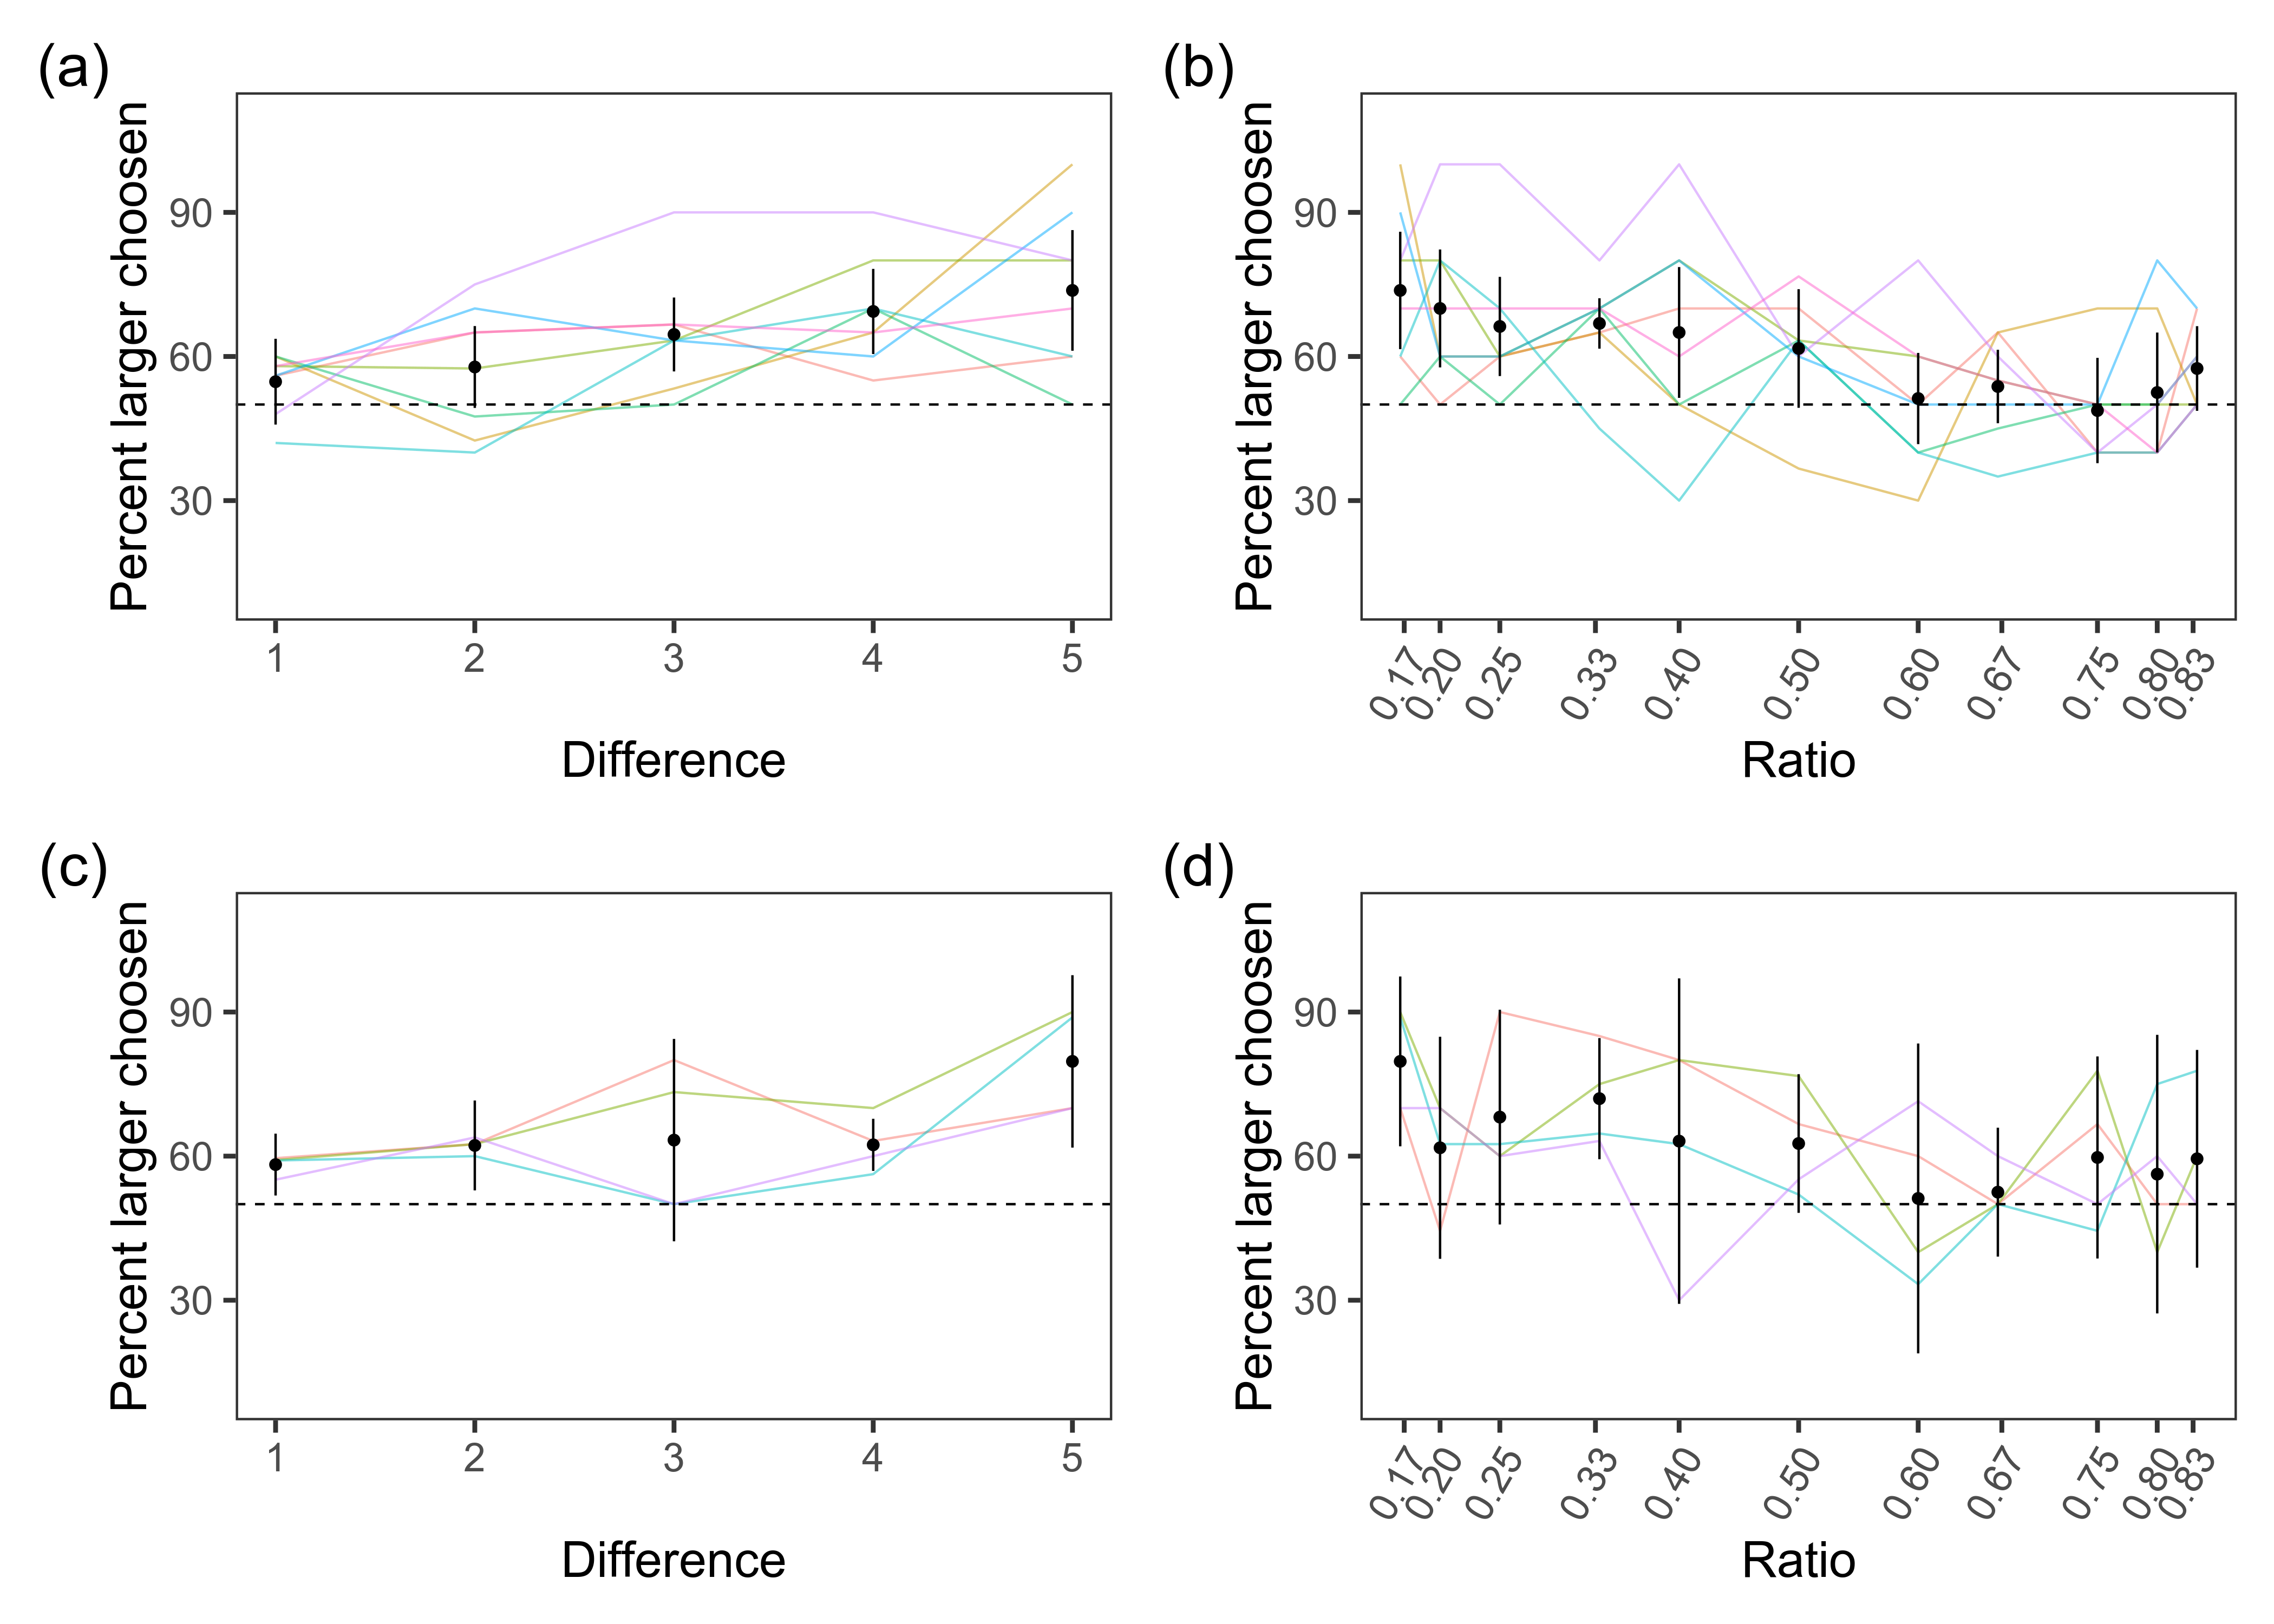
\includegraphics[width=1\linewidth]{../figures/food_figure} 

}

\caption{Food study difference \& ratio results for both replicate 1 and 2. For all four graphs mean preference for the larger option is shown on the y axis with the numerical difference or ratio options on the x axis. (a) Preference for larger ratios replicate 1. (b) Preference for larger differences replicate 1. (c) Preference for larger ratios replicate 2. (d) Preference for larger differences replicate 2. Dots represent mean values across all subjects and trials and error bars represent 95\% within-subject confidence intervals. Lines represent individual birds.}\label{fig:foodgraphs}
\end{figure}

\hypertarget{social-experiment-1}{%
\subsection{Social Experiment}\label{social-experiment-1}}

Hypothesis 1 predicted that subjects would choose the larger number of flock mates over the smaller. One sample t-tests provided moderate evidence that our hypothesis was supported during the first replicate (\(M = 55.33\), 95\% CI \([52.34, 58.32]\), \(t(9) = 4.03\), \(p = .003\), \(\mathrm{BF}_{\textrm{10}} = 16.67\)). However, evidence supported no difference from chance in the second replicate (\(M = 55.33\), 95\% CI \([52.34, 58.32]\), \(t(9) = 4.03\), \(p = .003\), \(\mathrm{BF}_{\textrm{10}} = 16.67\)). This is the only incongruency between the replicates and can most likely be accounted for that the slight preference for the larger side is not a true preference for larger \emph{amounts} but that a preferred partner is more likely to appear in the larger group. This was accounted for in replicate 2 with completing 10 replications of each pair instead of 5.

For hypotheses 2 and 3, we tested all possible random effects (subject, pair, and both) against the intercept only model to determine which of these random effects should be included in the full model. The data again supported the same best fitting model structure for both replicates of data: no random effect structure. For fixed effects, the intercept only model (Replicate 1: \(\mathrm{BF}_{\textrm{10}} = 0.07\), Replicate 2:\(\mathrm{BF}_{\textrm{10}} = 0.04\)) again best fit the data, suggesting that neither ratio nor difference influenced choice. Because ratio and difference failed to predict choices, neither of our hypothesis were supported by the data (Figure \ref{fig:socialgraphs}).



\begin{figure}

{\centering 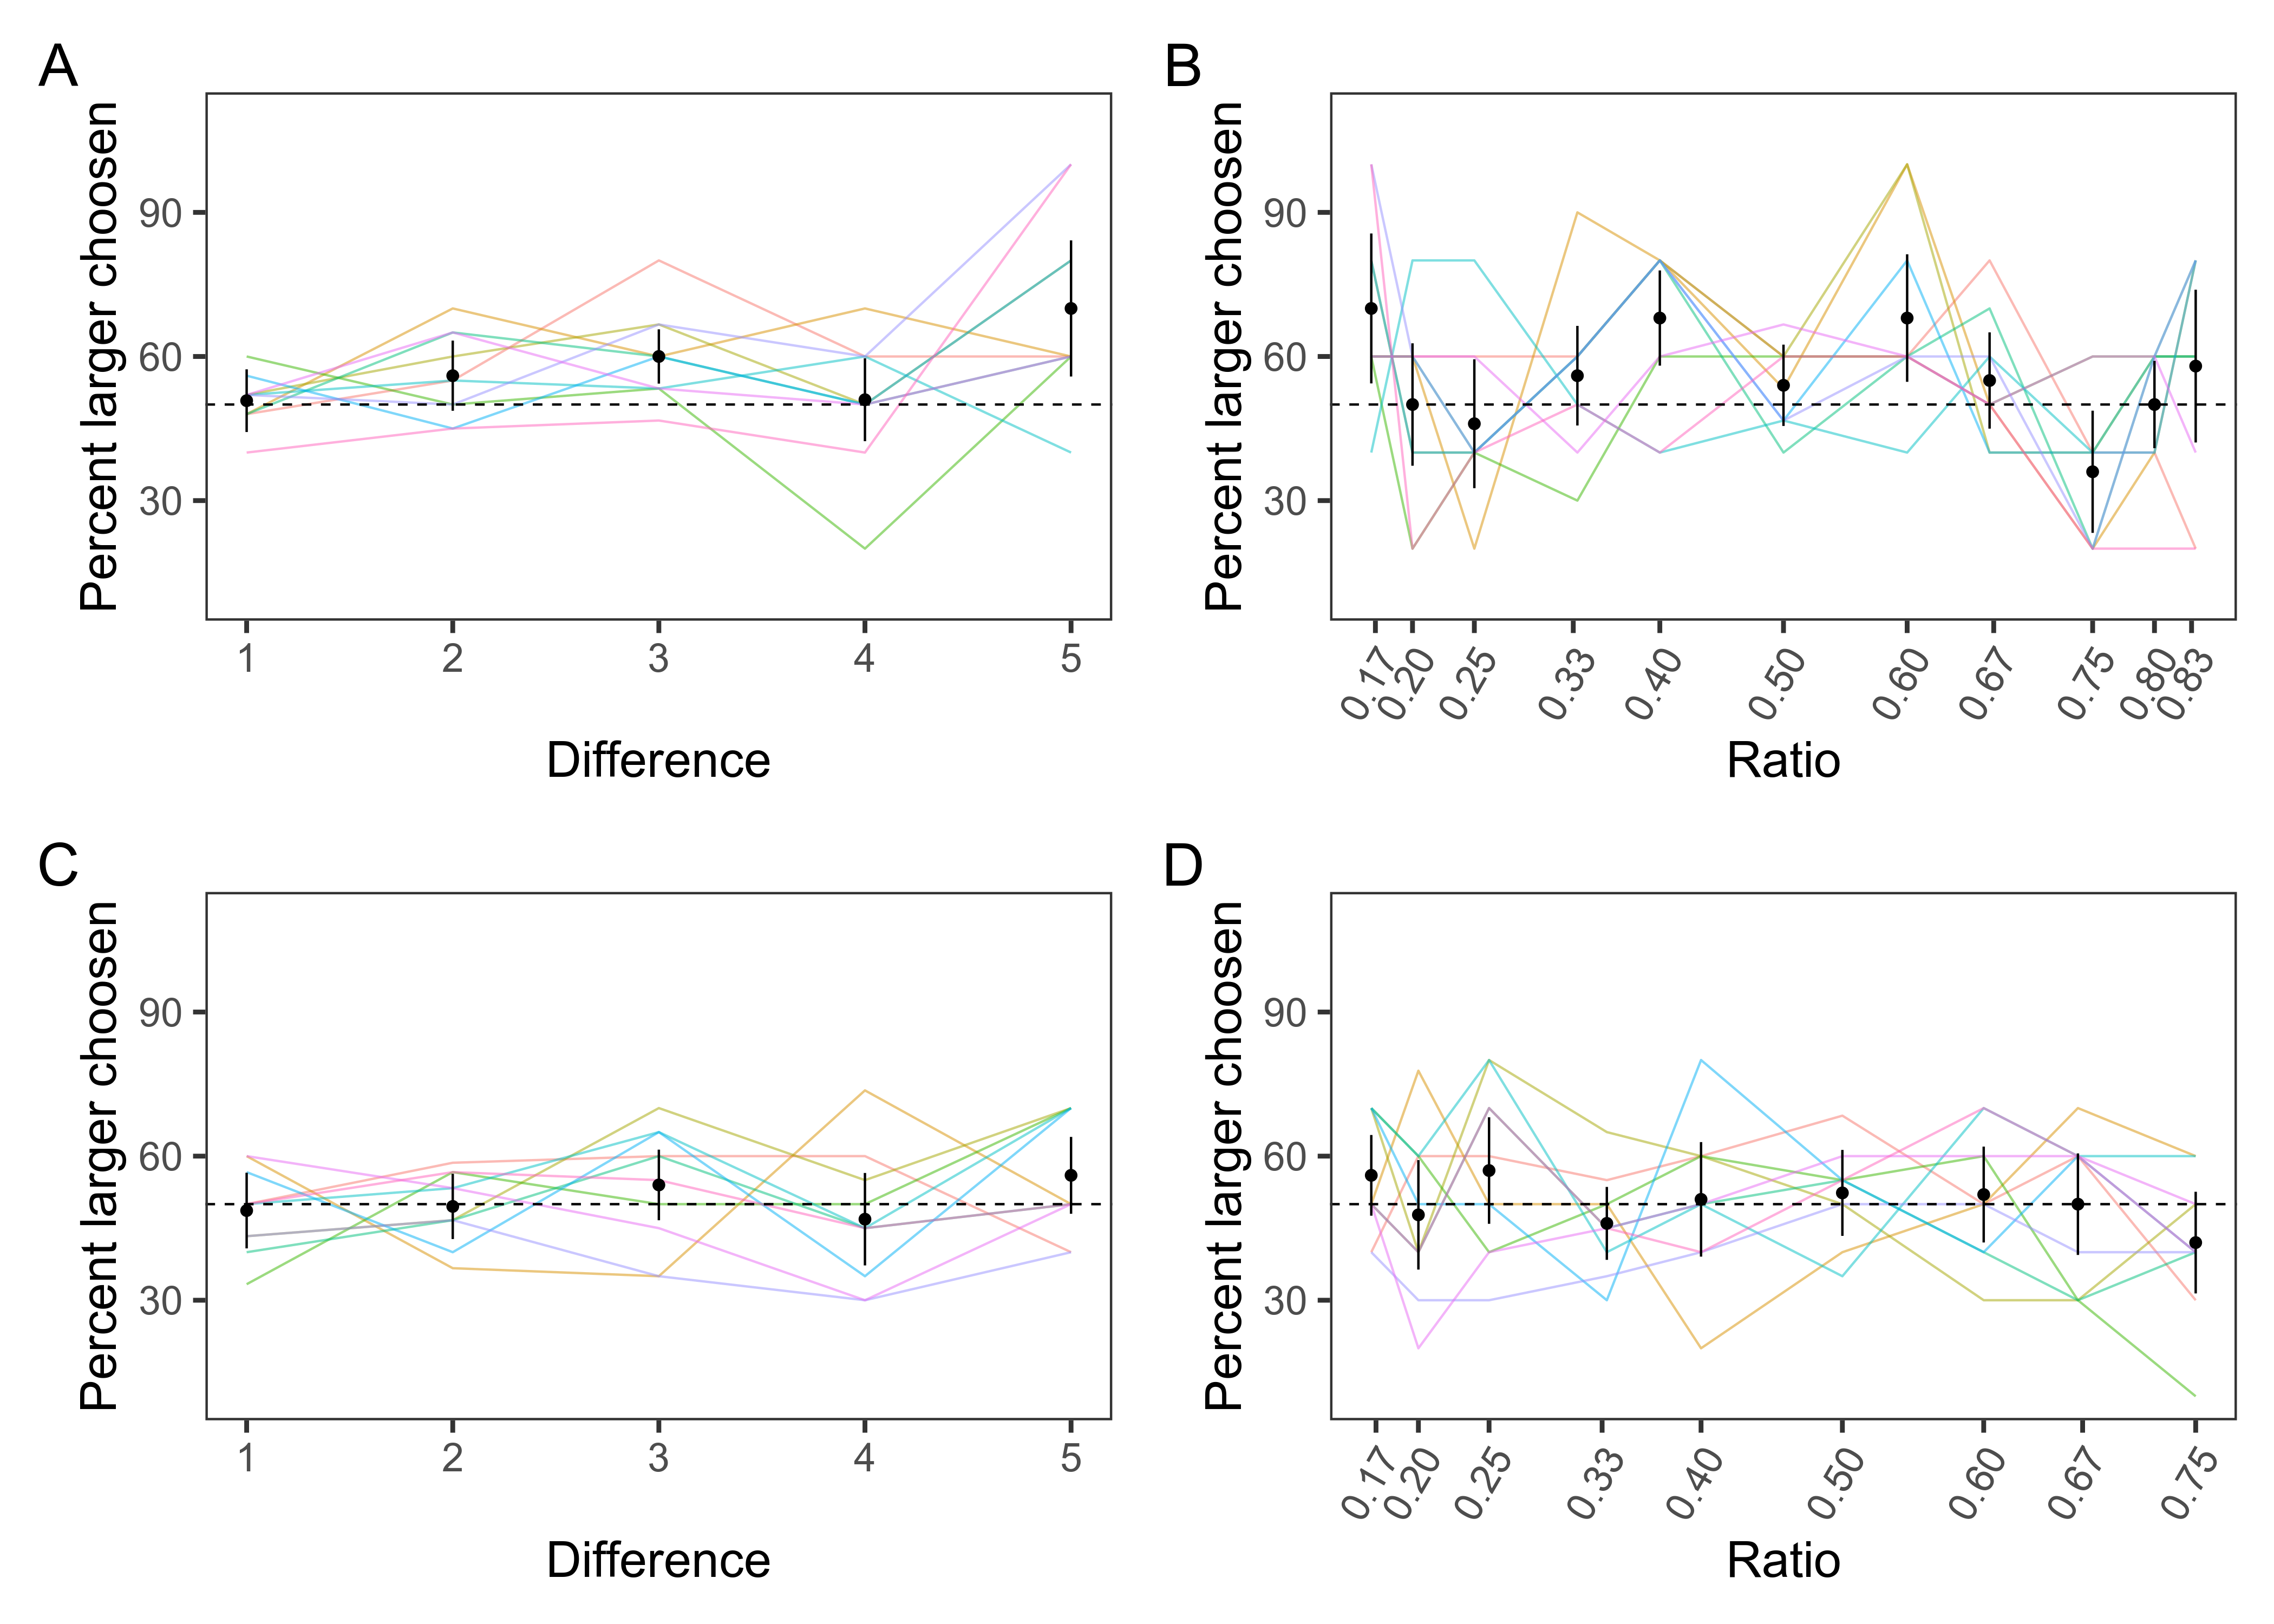
\includegraphics[width=1\linewidth]{../figures/social_figure} 

}

\caption{Social study difference \& ratio results for both replicate 1 and 2. For all four graphs mean preference for the larger option is shown on the y axis with the numerical difference or ratio options on the x axis. (a) Preference for larger ratios replicate 1. (b) Preference for larger differences replicate 1. (c) Preference for larger ratios replicate 2. (d) Preference for larger differences replicate 2. Dots represent mean values across all subjects and trials and error bars represent 95\% within-subject confidence intervals. Lines represent individual birds.}\label{fig:socialgraphs}
\end{figure}

\hypertarget{discussion}{%
\section{Discussion}\label{discussion}}

We examined pinyon jays' quantitative abilities in choosing between different numbers of food items and social partners. Over all numerical pairs, birds chose the larger of the two options in the food experiment but not in the social experiment, partially confirming our first hypothesis. In the food study, smaller numerical ratios but not larger numerical differences predicted the birds' choices, partially confirming our second hypothesis. In the social experiment, neither ratio nor difference predicted choice, contradicting our second hypothesis. In both the food and social experiments, difference and ratio did not independently predict choice, contradicting our third hypothesis.

In the food study, our pinyon jays preferred larger over smaller quantities more as the numerical ratios decrease, which aligns with previous corvid research demonstrating a numerical magnitude effect {[}20,24,31{]}. This provides evidence for pinyon jays using the approximate number system as a mechanism for quantification. However, unlike the previous corvid studies, we did not find the numerical distance effect, as number preference did not depend on the difference between two values.

In the social study, neither ratio nor difference predicted choice, suggesting that pinyon jays do not employ a single mechanism across object types. This outcome is surprising, as previous quantification tasks with conspecifics in fish found effects of difference and ratio {[}2,3{]}. It also suggests that the mechanisms underlying quantification in food and social partners differ.

The differences in numerical preference between food and social contexts may be due to different selective pressures. Both flock size and foraging techniques have consequences for evolutionary fitness, but they tackle different adaptive problems. Food consumption acts primarily via natural selection by enhancing survival. Flock size, however, is integral to both natural and sexual selection: natural selection in the form of predator avoidance and sexual selection in the form of mate preference. Joining a larger flock size allows an animal to dilute their chances of being eaten by predators (i.e., the dilution effect) but also may provide a larger pool of potential mates. For food items and social partners used to dilute predation risk, only number matters. But for mate preference or other social preferences, the identity of the partners matter. One possible explanation for the lack of a ratio or difference effect for the social preference task is that individual identity of birds overrides the importance of number. In fact, a follow-up analysis of our data showed wide variation in preferences for groups that contained the different stooge birds (Table ??). Pinyon jays have complex, long-term bonds with other flock members and mates {[}40{]}, which may make identity of group mates more important than sheer numbers.

Moreover, the birds in our studies did not experience signals of predation danger during the experiment and have not faced predation pressure in years. Without pressure to dilute risk in larger groups, the birds may have ignored group size, allowing them to use other information such as social partner identity to determine choice.

Our study design does not allow us to pinpoint the exact features by which the birds make these quantitative choices. For the food preference tasks, the birds may choose larger \emph{numbers} of food items or larger \emph{amounts} of them. Using number involves tracking the quantity of individuated objects. However, in many cases, animals choose based on amount, which refers to other measures or proxies of quantity such as item size, surface area, volume, perimeter, and density {[}41,42,\textbf{Menzel.1960?},\textbf{Uller.eteal.2003?}{]}. It is possible that our jays used, for example, surface area to choose their food items. This is a reasonable criteria because surface area may be a better proxy of total calories than absolute number (i.e., two large mealworms my provide more calories than three small mealworms). Future work is needed to tease apart which features birds use to make quantitative decisions.

\hypertarget{conclusion}{%
\subsection{Conclusion}\label{conclusion}}

This research investigated how pinyon jays assess numbers of food items and conspecifics in preference tasks. For food items, numerical ratio predicted their choices, but neither ratio nor difference predicted choices in the social preferences task. Though quantity is important for selecting food items, other factors such as flock mate identity may be more important for selecting social groups to join. Thus, in quantification situations, the type of objects to be quantified can drive the cognitive strategies that animals use.

\hypertarget{acknowledgments}{%
\subsection{Acknowledgments}\label{acknowledgments}}

This research was funded by National Science Foundation grants (NSF-1062045,
NSF-1658837). We would like to thank Kylie Hughes and Katie Carey for caring for our birds and Toria Biancalana, Hailey Wilson, Bailey Wilson, Isaac Martinez, and Rachel Bruner for helping run the experiments.

\hypertarget{ethics-approval}{%
\subsection{Ethics approval}\label{ethics-approval}}

All procedures were conducted in an ethical and responsible manner, in full compliance with all relevant codes of experimentation and legislation and were approved by the UNL Internal Review Board (protocol \# 17922) and Institutional Animal Care and Use Committee (protocol \# 1621).

\newpage

\hypertarget{references}{%
\section{References}\label{references}}

\hypertarget{refs}{}
\begin{CSLReferences}{0}{0}
\leavevmode\vadjust pre{\hypertarget{ref-Dacke.Srinivasan.2008}{}}%
\CSLLeftMargin{1. }%
\CSLRightInline{Dacke M, Srinivasan MV. 2008 Evidence for counting in insects. \emph{Animal Cognition} \textbf{11}, 683--689. (doi:\href{https://doi.org/10.1007/s10071-008-0159-y}{10.1007/s10071-008-0159-y})}

\leavevmode\vadjust pre{\hypertarget{ref-Agrillo.etal.2008}{}}%
\CSLLeftMargin{2. }%
\CSLRightInline{Agrillo C, Dadda M, Serena G, Bisazza A. 2008 Do fish count? {Spontaneous} discrimination of quantity in female mosquitofish. \emph{Animal Cognition} \textbf{11}, 495--503. (doi:\href{https://doi.org/10.1007/s10071-008-0140-9}{10.1007/s10071-008-0140-9})}

\leavevmode\vadjust pre{\hypertarget{ref-Agrillo.Dadda.2007}{}}%
\CSLLeftMargin{3. }%
\CSLRightInline{Agrillo C, Dadda M. 2007 Discrimination of the larger shoal in the poeciliid fish {Girardinus} falcatus. \emph{Ethology Ecology \& Evolution} \textbf{19}, 145--157. (doi:\href{https://doi.org/10.1080/08927014.2007.9522574}{10.1080/08927014.2007.9522574})}

\leavevmode\vadjust pre{\hypertarget{ref-Agrillo.etal.2011}{}}%
\CSLLeftMargin{4. }%
\CSLRightInline{Agrillo C, Piffer L, Bisazza A. 2011 Number versus continuous quantity in numerosity judgments by fish. \emph{Cognition} \textbf{119}, 281--287. (doi:\href{https://doi.org/10.1016/j.cognition.2010.10.022}{10.1016/j.cognition.2010.10.022})}

\leavevmode\vadjust pre{\hypertarget{ref-Uller.etal.2003}{}}%
\CSLLeftMargin{5. }%
\CSLRightInline{Uller C, Jaeger R, Guidry G, Martin C. 2003 Salamanders ({Plethodon} cinereus) go for more: Rudiments of number in an amphibian. \emph{Animal Cognition} \textbf{6}, 105--112. (doi:\href{https://doi.org/10.1007/s10071-003-0167-x}{10.1007/s10071-003-0167-x})}

\leavevmode\vadjust pre{\hypertarget{ref-Xia.etal.2001}{}}%
\CSLLeftMargin{6. }%
\CSLRightInline{Xia L, Emmerton J, Siemann M, Delius JD. 2001 Pigeons ({Columba} livia) learn to link numerosities with symbols. \emph{Journal of Comparative Psychology (Washington, D.C.: 1983)} \textbf{115}, 83--91. (doi:\href{https://doi.org/10.1037/0735-7036.115.1.83}{10.1037/0735-7036.115.1.83})}

\leavevmode\vadjust pre{\hypertarget{ref-Emmerton.Renner.2006}{}}%
\CSLLeftMargin{7. }%
\CSLRightInline{Emmerton J, Renner JC. 2006 Scalar effects in the visual discrimination of numerosity by pigeons. \emph{Learning \& Behavior} \textbf{34}, 176--192. (doi:\href{https://doi.org/10.3758/BF03193193}{10.3758/BF03193193})}

\leavevmode\vadjust pre{\hypertarget{ref-Emmerton.Renner.2009}{}}%
\CSLLeftMargin{8. }%
\CSLRightInline{Emmerton J, Renner JC. 2009 Local rather than global processing of visual arrays in numerosity discrimination by pigeons ({Columba} livia). \emph{Animal Cognition} \textbf{12}, 511--526. (doi:\href{https://doi.org/10.1007/s10071-009-0212-5}{10.1007/s10071-009-0212-5})}

\leavevmode\vadjust pre{\hypertarget{ref-Vonk.Beran.2012}{}}%
\CSLLeftMargin{9. }%
\CSLRightInline{Vonk J, Beran MJ. 2012 Bears {`count'} too: Quantity estimation and comparison in black bears, {Ursus} americanus. \emph{Animal Behaviour} \textbf{84}, 231--238. (doi:\href{https://doi.org/10.1016/j.anbehav.2012.05.001}{10.1016/j.anbehav.2012.05.001})}

\leavevmode\vadjust pre{\hypertarget{ref-Nieder.2018}{}}%
\CSLLeftMargin{10. }%
\CSLRightInline{Nieder A. 2018 Evolution of cognitive and neural solutions enabling numerosity judgements: Lessons from primates and corvids. \emph{Philosophical Transactions of the Royal Society B: Biological Sciences} \textbf{373}, 20160514. (doi:\href{https://doi.org/10.1098/rstb.2016.0514}{10.1098/rstb.2016.0514})}

\leavevmode\vadjust pre{\hypertarget{ref-Call.2000}{}}%
\CSLLeftMargin{11. }%
\CSLRightInline{Call J. 2000 Estimating and operating on discrete quantities in {Orangutans} ({Pongo} pygmaeus). \emph{Journal of Comparative Psychology} \textbf{114}, 136--147. (doi:\href{https://doi.org/10.1037/0735-7036.114.2.136}{10.1037/0735-7036.114.2.136})}

\leavevmode\vadjust pre{\hypertarget{ref-Beran.2001}{}}%
\CSLLeftMargin{12. }%
\CSLRightInline{Beran M. 2001 Summation and numerousness judgments of sequentially presented sets of items by chimpanzees ({Pan} troglodytes). \emph{Journal of comparative psychology (Washington, D.C. : 1983)} \textbf{115}, 181--91. (doi:\href{https://doi.org/10.1037//0735-7036.115.2.181}{10.1037//0735-7036.115.2.181})}

\leavevmode\vadjust pre{\hypertarget{ref-White.etal.2009}{}}%
\CSLLeftMargin{13. }%
\CSLRightInline{White DJ, Ho L, Freed-Brown G. 2009 Counting {Chicks} {Before} {They} {Hatch}: {Female} {Cowbirds} {Can} {Time} {Readiness} of a {Host} {Nest} for {Parasitism}. \emph{Psychological Science} \textbf{20}, 1140--1145. (doi:\href{https://doi.org/10.1111/j.1467-9280.2009.02418.x}{10.1111/j.1467-9280.2009.02418.x})}

\leavevmode\vadjust pre{\hypertarget{ref-Carazo.etal.2012}{}}%
\CSLLeftMargin{14. }%
\CSLRightInline{Carazo P, Fernández-Perea R, Font E. 2012 Quantity {Estimation} {Based} on {Numerical} {Cues} in the {Mealworm} {Beetle} ({Tenebrio} molitor). \emph{Frontiers in Psychology} \textbf{3}, 502. (doi:\href{https://doi.org/10.3389/fpsyg.2012.00502}{10.3389/fpsyg.2012.00502})}

\leavevmode\vadjust pre{\hypertarget{ref-Arak.1983}{}}%
\CSLLeftMargin{15. }%
\CSLRightInline{Arak A. 1983 Vocal interactions, call matching and territoriality in a {Sri} {Lankan} treefrog, {Philautus} leucorhinus ({Rhacophoridae}). \emph{Animal Behaviour} \textbf{31}, 292--302. (doi:\href{https://doi.org/10.1016/S0003-3472(83)80199-7}{10.1016/S0003-3472(83)80199-7})}

\leavevmode\vadjust pre{\hypertarget{ref-Nieder.2020}{}}%
\CSLLeftMargin{16. }%
\CSLRightInline{Nieder A. 2020 The {Adaptive} {Value} of {Numerical} {Competence}. \emph{Trends in Ecology \& Evolution} \textbf{35}, 605--617. (doi:\href{https://doi.org/10.1016/j.tree.2020.02.009}{10.1016/j.tree.2020.02.009})}

\leavevmode\vadjust pre{\hypertarget{ref-Agrillo.etal.2017}{}}%
\CSLLeftMargin{17. }%
\CSLRightInline{Agrillo C, Miletto Petrazzini ME, Bisazza A. 2017 Numerical abilities in fish: {A} methodological review. \emph{Behavioural Processes} \textbf{141}, 161--171. (doi:\href{https://doi.org/10.1016/j.beproc.2017.02.001}{10.1016/j.beproc.2017.02.001})}

\leavevmode\vadjust pre{\hypertarget{ref-Yang.Chiao.2016}{}}%
\CSLLeftMargin{18. }%
\CSLRightInline{Yang T-I, Chiao C-C. 2016 Number sense and state-dependent valuation in cuttlefish. \emph{Proceedings of the Royal Society B: Biological Sciences} \textbf{283}, 20161379. (doi:\href{https://doi.org/10.1098/rspb.2016.1379}{10.1098/rspb.2016.1379})}

\leavevmode\vadjust pre{\hypertarget{ref-Feigenson.etal.2004}{}}%
\CSLLeftMargin{19. }%
\CSLRightInline{Feigenson L, Dehaene S, Spelke E. 2004 Core systems of number. \emph{Trends in Cognitive Sciences} \textbf{8}, 307--314. (doi:\href{https://doi.org/10.1016/j.tics.2004.05.002}{10.1016/j.tics.2004.05.002})}

\leavevmode\vadjust pre{\hypertarget{ref-Ditz.Nieder.2016}{}}%
\CSLLeftMargin{20. }%
\CSLRightInline{Ditz HM, Nieder A. 2016 Numerosity representations in crows obey the {Weber}--{Fechner} law. \emph{Proceedings of the Royal Society B: Biological Sciences} \textbf{283}, 20160083. (doi:\href{https://doi.org/10.1098/rspb.2016.0083}{10.1098/rspb.2016.0083})}

\leavevmode\vadjust pre{\hypertarget{ref-Dehaene.etal.1998}{}}%
\CSLLeftMargin{21. }%
\CSLRightInline{Dehaene S, Dehaene-Lambertz G, Cohen L. 1998 Abstract representations of numbers in the animal and human brain. \emph{Trends in Neurosciences} \textbf{21}, 355--361. (doi:\href{https://doi.org/10.1016/S0166-2236(98)01263-6}{10.1016/S0166-2236(98)01263-6})}

\leavevmode\vadjust pre{\hypertarget{ref-Agrillo.Beran.2013}{}}%
\CSLLeftMargin{22. }%
\CSLRightInline{Agrillo C, Beran MJ. 2013 \href{https://www.academia.edu/6879466/Number_without_language_comparative_psychology_and_the_evolution_of_numerical_cognition}{Number without language: Comparative psychology and the evolution of numerical cognition}. \emph{Frontiers in psychology} }

\leavevmode\vadjust pre{\hypertarget{ref-Agrillo.Bisazza.2014}{}}%
\CSLLeftMargin{23. }%
\CSLRightInline{Agrillo C, Bisazza A. 2014 Spontaneous versus trained numerical abilities. {A} comparison between the two main tools to study numerical competence in non-human animals. \emph{Journal of Neuroscience Methods} \textbf{234}, 82--91. (doi:\href{https://doi.org/10.1016/j.jneumeth.2014.04.027}{10.1016/j.jneumeth.2014.04.027})}

\leavevmode\vadjust pre{\hypertarget{ref-Kelly.2016}{}}%
\CSLLeftMargin{24. }%
\CSLRightInline{Kelly EM. 2016 Counting on your friends: {The} role of social environment on quantity discrimination. \emph{Behavioural Processes} \textbf{128}, 9--16. (doi:\href{https://doi.org/10.1016/j.beproc.2016.03.019}{10.1016/j.beproc.2016.03.019})}

\leavevmode\vadjust pre{\hypertarget{ref-Scarf.etal.2011}{}}%
\CSLLeftMargin{25. }%
\CSLRightInline{Scarf D, Hayne H, Colombo M. 2011 Pigeons on {Par} with {Primates} in {Numerical} {Competence}. \emph{Science} (doi:\href{https://doi.org/10.1126/science.1213357}{10.1126/science.1213357})}

\leavevmode\vadjust pre{\hypertarget{ref-Rugani.etal.2013}{}}%
\CSLLeftMargin{26. }%
\CSLRightInline{Rugani R, Cavazzana A, Vallortigara G, Regolin L. 2013 One, two, three, four, or is there something more? {Numerical} discrimination in day-old domestic chicks. \emph{Animal Cognition} \textbf{16}, 557--564. (doi:\href{https://doi.org/10.1007/s10071-012-0593-8}{10.1007/s10071-012-0593-8})}

\leavevmode\vadjust pre{\hypertarget{ref-Cantlon.Brannon.2006}{}}%
\CSLLeftMargin{27. }%
\CSLRightInline{Cantlon JF, Brannon EM. 2006 Shared {System} for {Ordering} {Small} and {Large} {Numbers} in {Monkeys} and {Humans}. \emph{Psychological Science} \textbf{17}, 401--406. (doi:\href{https://doi.org/10.1111/j.1467-9280.2006.01719.x}{10.1111/j.1467-9280.2006.01719.x})}

\leavevmode\vadjust pre{\hypertarget{ref-Merten.Nieder.2009}{}}%
\CSLLeftMargin{28. }%
\CSLRightInline{Merten K, Nieder A. 2009 Compressed scaling of abstract numerosity representations in adult humans and monkeys. \emph{Journal of Cognitive Neuroscience} \textbf{21}, 333--346. (doi:\href{https://doi.org/10.1162/jocn.2008.21032}{10.1162/jocn.2008.21032})}

\leavevmode\vadjust pre{\hypertarget{ref-Hanus.Call.2007}{}}%
\CSLLeftMargin{29. }%
\CSLRightInline{Hanus D, Call J. 2007 Discrete quantity judgments in the great apes ({Pan} paniscus, {Pan} troglodytes, {Gorilla} gorilla, {Pongo} pygmaeus): {The} effect of presenting whole sets versus item-by-item. \emph{Journal of Comparative Psychology} \textbf{121}, 241--249. (doi:\href{https://doi.org/10.1037/0735-7036.121.3.241}{10.1037/0735-7036.121.3.241})}

\leavevmode\vadjust pre{\hypertarget{ref-Evans.etal.2009}{}}%
\CSLLeftMargin{30. }%
\CSLRightInline{Evans TA, Beran MJ, Harris EH, Rice DF. 2009 Quantity judgments of sequentially presented food items by capuchin monkeys ({Cebus} apella). \emph{Animal Cognition} \textbf{12}, 97--105. (doi:\href{https://doi.org/10.1007/s10071-008-0174-z}{10.1007/s10071-008-0174-z})}

\leavevmode\vadjust pre{\hypertarget{ref-Tornick.etal.2015}{}}%
\CSLLeftMargin{31. }%
\CSLRightInline{Tornick JK, Callahan ES, Gibson BM. 2015 An investigation of quantity discrimination in {Clark}'s nutcrackers ({Nucifraga} columbiana). \emph{Journal of Comparative Psychology (Washington, D.C.: 1983)} \textbf{129}, 17--25. (doi:\href{https://doi.org/10.1037/a0037863}{10.1037/a0037863})}

\leavevmode\vadjust pre{\hypertarget{ref-Ditz.Nieder.2015}{}}%
\CSLLeftMargin{32. }%
\CSLRightInline{Ditz HM, Nieder A. 2015 Neurons selective to the number of visual items in the corvid songbird endbrain. \emph{Proceedings of the National Academy of Sciences} \textbf{112}, 7827--7832. (doi:\href{https://doi.org/10.1073/pnas.1504245112}{10.1073/pnas.1504245112})}

\leavevmode\vadjust pre{\hypertarget{ref-Buckingham.etal.2007}{}}%
\CSLLeftMargin{33. }%
\CSLRightInline{Buckingham JN, Wong BBM, Rosenthal GG. 2007 Shoaling decisions in female swordtails: {How} do fish gauge group size? \emph{Behaviour} \textbf{144}, 1333--1346. (doi:\href{https://doi.org/10.1163/156853907782418196}{10.1163/156853907782418196})}

\leavevmode\vadjust pre{\hypertarget{ref-Gomez-Laplaza.Gerlai.2016}{}}%
\CSLLeftMargin{34. }%
\CSLRightInline{Gómez-Laplaza LM, Gerlai R. 2016 Discrimination of large quantities: {Weber}'s law and short-term memory in angelfish, {Pterophyllum} scalare. \emph{Animal Behaviour} \textbf{112}, 29--37. (doi:\href{https://doi.org/10.1016/j.anbehav.2015.10.022}{10.1016/j.anbehav.2015.10.022})}

\leavevmode\vadjust pre{\hypertarget{ref-Krause.Ruxton.2002}{}}%
\CSLLeftMargin{35. }%
\CSLRightInline{Krause J, Ruxton GD. 2002 \emph{Living in {Groups}}. OUP Oxford. }

\leavevmode\vadjust pre{\hypertarget{ref-Silk.etal.2014}{}}%
\CSLLeftMargin{36. }%
\CSLRightInline{Silk MJ, Croft DP, Tregenza T, Bearhop S. 2014 The importance of fission--fusion social group dynamics in birds. \emph{Ibis} \textbf{156}, 701--715. (doi:\href{https://doi.org/10.1111/ibi.12191}{10.1111/ibi.12191})}

\leavevmode\vadjust pre{\hypertarget{ref-Gomez-Laplaza.Gerlai.2011}{}}%
\CSLLeftMargin{37. }%
\CSLRightInline{Gómez-Laplaza LM, Gerlai R. 2011 Can angelfish ({Pterophyllum} scalare) count? {Discrimination} between different shoal sizes follows {Weber}'s law. \emph{Animal Cognition} \textbf{14}, 1--9. (doi:\href{https://doi.org/10.1007/s10071-010-0337-6}{10.1007/s10071-010-0337-6})}

\leavevmode\vadjust pre{\hypertarget{ref-R-base}{}}%
\CSLLeftMargin{38. }%
\CSLRightInline{R Core Team. 2021 \emph{R: A language and environment for statistical computing}. Vienna, Austria: R Foundation for Statistical Computing. See \url{https://www.R-project.org/}.}

\leavevmode\vadjust pre{\hypertarget{ref-R-BayesFactor}{}}%
\CSLLeftMargin{39. }%
\CSLRightInline{Morey RD, Rouder JN. 2018 \emph{BayesFactor: Computation of bayes factors for common designs}. See \url{https://CRAN.R-project.org/package=BayesFactor}.}

\leavevmode\vadjust pre{\hypertarget{ref-Marzluff.Balda.1992}{}}%
\CSLLeftMargin{40. }%
\CSLRightInline{Marzluff JM, Balda RP. 1992 \emph{The {Pinyon} {Jay}: {Behavioral} {Ecology} of a {Colonial} and {Cooperative} {Corvid}}. First Edition. London: Academic Press. }

\leavevmode\vadjust pre{\hypertarget{ref-Stevens.etal.2007}{}}%
\CSLLeftMargin{41. }%
\CSLRightInline{Stevens JR, Wood JN, Hauser MD. 2007 When quantity trumps number: Discrimination experiments in cotton-top tamarins ({Saguinus} oedipus) and common marmosets ({Callithrix} jacchus). \emph{Animal Cognition} \textbf{10}, 429--437. (doi:\href{https://doi.org/10.1007/s10071-007-0081-8}{10.1007/s10071-007-0081-8})}

\leavevmode\vadjust pre{\hypertarget{ref-Gomez-Laplaza.etal.2019}{}}%
\CSLLeftMargin{42. }%
\CSLRightInline{Gómez-Laplaza LM, Romero L, Gerlai R. 2019 The role of item size on choosing contrasted food quantities in angelfish ({Pterophyllum} scalare). \emph{Scientific Reports} \textbf{9}, 15305. (doi:\href{https://doi.org/10.1038/s41598-019-51753-1}{10.1038/s41598-019-51753-1})}

\end{CSLReferences}


\end{document}
